\section{Vectors, mappings, and matrices}
\label{vecsandmaps:section}

\LAtt{A.1}

\LO{
\item Express n-tuples of numbers as vectors,
\item Perform operations on vectors, and
\item Understand how linear maps on vectors give rise to matrices. 
}

% \sectionnotes{2 lectures}

In real life, there is most often more than one variable.
We wish to organize dealing with multiple variables in a consistent
manner, and in particular organize dealing with linear equations and linear
mappings, as those both rather useful and rather easy to handle.
Mathematicians joke that
\myquote{to an engineer every problem is linear, and everything is a
matrix.}
And well, they (the engineers) are not wrong. 
Quite often, solving an engineering problem is figuring out the
right finite-dimensional linear problem to solve, which is then
solved with some matrix manipulation.
Most importantly, linear problems are the ones that we know how to solve,
and we have many tools to solve them.
For engineers, mathematicians, physicists, and anybody in a technical
field it is absolutely vital to learn linear algebra.

As motivation, suppose we wish to solve
\begin{equation*}
\begin{aligned}
& x-y = 2 , \\
& 2x+y = 4 ,
\end{aligned}
\end{equation*}
for $x$ and $y$, that is, find numbers $x$ and $y$ such that the two
equations are satisfied.
Let us perhaps start by adding the equations together to find
\begin{equation*}
x+2x-y+y = 2+4, \qquad \text{or} \qquad 3x = 6 .
\end{equation*}
In other words, $x=2$.  Once we have that, we plug in $x=2$ into the
first equation to find $2-y=2$, so $y=0$.  OK\@, that was easy.  What is all
this fuss about linear equations.  Well, try doing this if you have
5000 unknowns\footnote{One of the downsides of making everything look like a
linear problem is that the number of variables tends to become huge.}.
Also, we may have such equations not of just numbers,
but of functions and derivatives of functions in differential equations.
Clearly we need a more systematic way of doing things.
A nice consequence of making things systematic and simpler to write down
is that it becomes easier to have computers do the work for us.
Computers are rather stupid, they do not think,
but are very good at doing lots of repetitive
tasks precisely, as long as we figure out a systematic way for them to
perform the tasks.

\subsection{Vectors and operations on vectors}

Consider $n$ real numbers as an $n$-tuple:
\begin{equation*}
(x_1,x_2,\ldots,x_n). 
\end{equation*}
The set of such $n$-tuples is the so-called
\emph{$n$-dimensional space}\index{n-dimensional space@$n$-dimensional space},
often denoted by ${\mathbb R}^n$.
Sometimes we call this the $n$-dimensional
\emph{\myindex{euclidean space}}%
\footnote{Named after the ancient Greek mathematician
\href{https://en.wikipedia.org/wiki/Euclid}{Euclid of Alexandria}
(around 300 BC), possibly the most famous of mathematicians; even
small towns often have Euclid Street or Euclid Avenue.}. 
In two dimensions, ${\mathbb R}^2$ is called the
\emph{\myindex{cartesian plane}}%
\footnote{Named after the French mathematician
\href{https://en.wikipedia.org/wiki/Descartes}{Ren\'e Descartes}
(1596--1650).  It is \myquote{cartesian} as his name in Latin is Renatus
Cartesius.}, and in three dimensions, it is the same \myquote{3-dimensional space} that is dealt with in multivariable calculus.
Each such $n$-tuple represents a point in the $n$-dimensional space.
For example, the point
$(1,2)$ in the plane ${\mathbb R}^2$
is one unit to the right and two units up from the
origin.

When we do algebra with these $n$-tuples of numbers we call them
\emph{vectors}\index{vector}\footnote{%
A common notation to distinguish vectors from points is to write $(1,2)$ 
for the point and $\langle 1,2 \rangle$ for the vector.  We write both as
$(1,2)$.}.  Mathematicians are keen on separating
what is a vector and what is a point of the space or in the plane,
and it turns out
to be an important distinction, however, for the purposes of linear algebra
we can think of everything being represented by a vector.
A way to think of a vector, which is especially useful in calculus
and differential equations, is an arrow.  It is an object that has
a \emph{\myindex{direction}} and a \emph{magnitude}.
For example, the vector $(1,2)$
is the arrow from the origin to the point $(1,2)$ in the plane.
The magnitude is the length of the arrow.
See \figurevref{linalg-vecarrow:fig}.
If we think of vectors as arrows,
the arrow doesn't always have to start at the origin.  If we do move it
around, however, it should always keep the same direction and the same magnitude.

\begin{myfig}
\capstart
\inputpdft{linalg-vecarrow}
\caption{The vector $(1,2)$ drawn as an arrow from the origin to the point
$(1,2)$.\label{linalg-vecarrow:fig}}
\end{myfig}

As vectors are arrows, when we want to give a name to a vector,
we draw a little arrow above it:
\begin{equation*}
\vec{x}
\end{equation*}
Another popular notation is $\mathbf{x}$, although we will use the little
arrows.  It may be easy to write a bold letter in a book, but it is not so
easy to write it by hand on paper or on the board.
Mathematicians often don't even write the arrows.  A mathematician would
write $x$ and just remember that $x$ is a vector and not a number.
Just like you remember that Bob is your uncle, and you don't have to
keep repeating \myquote{Uncle Bob} and you can just say \myquote{Bob.}
In this book, however, we will call Bob \myquote{Uncle Bob}
and write vectors with the little arrows.

The \emph{\myindex{magnitude}} can be computed using Pythagorean theorem.
The vector $(1,2)$ drawn in the figure has magnitude $\sqrt{1^2+2^2} =
\sqrt{5}$.  The magnitude is denoted by $\lVert \vec{x} \rVert$,
and, in any number of dimensions, it can be computed in the same way:
\begin{equation*}
\lVert \vec{x} \rVert
=
\lVert (x_1,x_2,\ldots,x_n) \rVert
=
\sqrt{x_1^2+x_2^2+\cdots+x_n^2} .
\end{equation*}

For reasons that will become clear in the next section, we often
write vectors as so-called
\emph{column vectors}\index{column vector}:
\begin{equation*}
\vec{x} = 
\begin{bmatrix}
x_{1} \\ x_2 \\ \vdots \\ x_n
\end{bmatrix} .
\end{equation*}
Don't worry.  It is just a different way of writing the same thing, and
it will be useful later.  For example, the vector $(1,2)$ can be written as
\begin{equation*}
\begin{bmatrix}
1 \\ 2
\end{bmatrix} .
\end{equation*}

\begin{mywrapfig}[15]{3.25in}
\capstart
\inputpdft{linalg-vecadd}
\caption{Adding the vectors $(1,2)$, drawn dotted, and $(2,-3)$, drawn dashed.  The
result, $(3,-1)$, is drawn as a solid arrow.\label{linalg-vecadd:fig}}
\end{mywrapfig}

The fact that we write arrows above vectors allows us to write several
vectors $\vec{x}_1$, $\vec{x}_2$, etc., without confusing these with the
components of some other vector $\vec{x}$.

So where is the \emph{algebra} from \emph{linear algebra}?
Well, arrows can be added, subtracted,
and multiplied by numbers.
First we consider \emph{addition}\index{adding vectors}.
If we have two arrows, we simply
move along one, and then along the other.  See
\figurevref{linalg-vecadd:fig}.

It is rather easy to see what it does to the numbers that represent the
vectors.  Suppose we want to add $(1,2)$ to $(2,-3)$ as in the figure.
So we travel along $(1,2)$
and then we travel along $(2,-3)$ in the sense of ``tip-to-tail'' addition that you may have seen in previous classes.
What we did was travel one unit right, two units up, and then
we travelled two units right, and three units down (the negative three).  That
means that we ended up at $\bigl(1+2,2+(-3)\bigr) = (3,-1)$.
And that's how addition always works:
\begin{equation*}
\begin{bmatrix}
x_{1} \\ x_2 \\ \vdots \\ x_n
\end{bmatrix} +
\begin{bmatrix}
y_{1} \\ y_2 \\ \vdots \\ y_n
\end{bmatrix} =
\begin{bmatrix}
x_1 + y_{1} \\ x_2+ y_2 \\ \vdots \\ x_n + y_n
\end{bmatrix} .
\end{equation*}

\begin{mywrapfig}[13]{3.25in}
\capstart
\inputpdft{linalg-vecsub}
\caption{Subtraction, the vector $(1,2)$, drawn dotted, minus $(-2,1)$,
drawn dashed.  The
result, $(3,1)$, is drawn as a solid arrow.\label{linalg-vecsub:fig}}
\end{mywrapfig}

\emph{Subtracting}\index{subtracting vectors} is similar.
What $\vec{x}- \vec{y}$ means visually is that
we first travel along $\vec{x}$, and then we travel
backwards along $\vec{y}$.
See \figurevref{linalg-vecsub:fig}.
It is like adding
$\vec{x}+ (- \vec{y})$ where $-\vec{y}$
is the arrow we obtain by erasing the arrow head
from one side and drawing it on the other side, that is, we reverse the
direction.  In terms of the numbers, we simply go backwards in both directions,
so we negate both numbers.  For example, if $\vec{y}$ is $(-2,1)$,
then $-\vec{y}$ is $(2,-1)$.

Another intuitive thing to do to a vector is to
\emph{scale}\index{scale a vector} it.
We represent this by multiplication of a number with a vector.
Because of this, when we wish to distinguish between vectors and numbers, we
call the numbers \emph{scalars}\index{scalar}.
For example,
suppose we want to travel three times further.  If the vector is $(1,2)$,
travelling 3 times further means going 3 units to the right and 6 units up,
so we get the vector $(3,6)$.
We just multiply each number in the vector by 3.
If $\alpha$ is a number, then
\begin{equation*}
\alpha
\begin{bmatrix}
x_{1} \\ x_2 \\ \vdots \\ x_n
\end{bmatrix} =
\begin{bmatrix}
\alpha x_{1} \\ \alpha x_2 \\ \vdots \\ \alpha x_n
\end{bmatrix} .
\end{equation*}
Scaling (by a positive number) multiplies the magnitude
and leaves direction untouched.
The magnitude of $(1,2)$
is $\sqrt{5}$.  The magnitude of 3 times $(1,2)$, that is, $(3,6)$, is
$3\sqrt{5}$.

When the scalar is negative, then when we multiply a vector by it, the
vector is not only scaled, but it also switches direction.
So
multiplying $(1,2)$ by $-3$ means we should go 3 times further but in the
opposite direction, so 3 units to the left and 6 units down, or in other
words, $(-3,-6)$.  As we mentioned above, $-\vec{y}$ is a reverse of
$\vec{y}$, and this is the same as $(-1)\vec{y}$.

In \figurevref{linalg-vecscale:fig}, you can see a couple of examples of
what scaling a vector means visually.

\begin{myfig}
\capstart
\inputpdft{linalg-vecscale}
\caption{A vector $\vec{x}$, the vector $2\vec{x}$ (same direction,
double the magnitude), and the vector $-1.5\vec{x}$ (opposite direction,
1.5 times the magnitude).\label{linalg-vecscale:fig}}
\end{myfig}

We put all of these operations together to work out more complicated expressions.
Let us compute a small example:
\begin{equation*}
3
\begin{bmatrix}
1 \\ 2
\end{bmatrix}
+
2
\begin{bmatrix}
-4 \\ -1
\end{bmatrix} 
-
3
\begin{bmatrix}
-2 \\ 2
\end{bmatrix} 
=
\begin{bmatrix}
3(1)+2(-4)-3(-2) \\ 3(2)+2(-1)-3(2)
\end{bmatrix}
=
\begin{bmatrix}
1 \\ -2
\end{bmatrix}
.
\end{equation*}

\medskip

As we said a vector is a direction and a magnitude.  Magnitude is easy to
represent, it is just a number.  The \emph{\myindex{direction}} is usually
given by a vector with magnitude one.  We call such a vector a
\emph{\myindex{unit vector}}.  That is, $\vec{u}$ is a unit vector when
$\lVert \vec{u} \rVert = 1$.  For example, the vectors $(1,0)$,
$(\nicefrac{1}{\sqrt{2}},\nicefrac{1}{\sqrt{2}})$, and $(0,-1)$ are all
unit vectors.

To represent the direction of a vector $\vec{x}$, we need to find the 
unit vector in the same direction.  To do so, we simply rescale
$\vec{x}$ by the reciprocal of the magnitude, that is
$\frac{1}{\lVert \vec{x} \rVert} \vec{x}$, or more concisely
$\frac{\vec{x}}{\lVert \vec{x} \rVert}$.

For example, the unit vector in the direction of $(1,2)$ is the vector
\begin{equation*}
\frac{1}{\sqrt{1^2+2^2}} (1,2)
=
\left( \frac{1}{\sqrt{5}}, \frac{2}{\sqrt{5}} \right) .
\end{equation*}



\subsubsection{Linear Combinations and Linear Independence}

If we have vectors of a given size (say a collection of 3 component vectors), there are only two different operations we can perform on them; adding them together and multiplying them by real numbers. While this may seem fairly limited, we can take a small number of vectors and generate a lot more vectors from them. By putting these operations together, we get the definition of a linear combination. 

\begin{definition}
Given row or column vectors $\vec{y}_1, \vec{y}_2, \ldots, \vec{y}_n$,
a \emph{\myindex{linear combination}} is an expression of the form
\begin{equation*}
\alpha_1 \vec{y}_1 + 
\alpha_2 \vec{y}_2 + 
\cdots +
\alpha_n \vec{y}_n ,
\end{equation*}
where $\alpha_1, \alpha_2, \ldots, \alpha_n$ are all scalars.
\end{definition}%
For example,
$3 \vec{y}_1 + \vec{y}_2 - 5 \vec{y}_3$ is a linear combination
of $\vec{y}_1$, $\vec{y}_2$, and $\vec{y}_3$. Another example is that $\left[\begin{smallmatrix} 2 \\ 3 \\ 4 \end{smallmatrix} \right]$ can be written as a linear combination of $\left[\begin{smallmatrix} 1 \\ 0 \\ 1 \end{smallmatrix}\right]$,\ $\left[\begin{smallmatrix} 0 \\ 1 \\ 2 \end{smallmatrix}\right]$, and $\left[\begin{smallmatrix}  0 \\ -1 \\ 2 \end{smallmatrix}\right]$ as 
\begin{equation*}
 \begin{bmatrix} 2 \\ 3 \\ 4 \end{bmatrix} = 2\begin{bmatrix}  1 \\ 0 \\ 1 \end{bmatrix} + 2 \begin{bmatrix} 0 \\ 1 \\ 2  \end{bmatrix} - \begin{bmatrix} 0 \\ -1 \\ 2 \end{bmatrix}.
 \end{equation*}

Given any collection of vectors $\vec{y}_1, \vec{y}_2, \ldots, \vec{y}_n$, it is always possible to write $\vec{0}$ as a linear combination of these vectors by choosing $\alpha_i = 0$ for all $i$. Then we are adding a bunch of zeros together and so get zero. However, this may not be the only way to get zero. Whether or not it is depends heavily on the exact vectors involved.

\begin{definition}
We say the vectors $\vec{y}_1$, $\vec{y}_2$, \ldots, $\vec{y}_n$ are
\emph{\myindex{linearly independent}} if the only way to pick $\alpha_1,\ \alpha_2, ..., \alpha_n$ to satisfy
\begin{equation*}
\alpha_1 \vec{x}_1 + 
\alpha_2 \vec{x}_2 + 
\cdots +
\alpha_n \vec{x}_n 
=
\vec{0}
\end{equation*}
is $\alpha_1 = \alpha_2 = \cdots = \alpha_n = 0$.
Otherwise, we say the vectors are \emph{\myindex{linearly dependent}}.
\end{definition}

\begin{example} The vectors
$\left[ \begin{smallmatrix} 1 \\ 2 \end{smallmatrix} \right]$
and
$\left[ \begin{smallmatrix} 0 \\ 1 \end{smallmatrix} \right]$
are linearly independent.
\end{example}

\begin{exampleSol}
Let's try:
\begin{equation*}
\alpha_1
\begin{bmatrix} 1 \\ 2 \end{bmatrix}
+
\alpha_2
\begin{bmatrix} 0 \\ 1 \end{bmatrix}
=
\begin{bmatrix} \alpha_1 \\ 2 \alpha_1 + \alpha_2 \end{bmatrix}
=
\vec{0} =
\begin{bmatrix} 0 \\ 0 \end{bmatrix} .
\end{equation*}
So $\alpha_1 = 0$, and then it is clear that $\alpha_2 = 0$ as well.  In
other words, the vectors are linearly independent.
\end{exampleSol}

If a set of vectors is linearly dependent, that is, we have an expression of the form
\begin{equation*}
\alpha_1\vec{x}_1 + \alpha_2\vec{x}_2 + \cdots + \alpha_n\vec{x}_n = 0
\end{equation*}
with some of the $\alpha_j$'s
are nonzero, then we can solve for one vector in terms of the others.
Suppose $\alpha_1 \not= 0$.  Since
$\alpha_1 \vec{x}_1 + 
\alpha_2 \vec{x}_2 + 
\cdots +
\alpha_n \vec{x}_n 
=
\vec{0}$, then
\begin{equation*}
\vec{x}_1 
=
\frac{-\alpha_2}{\alpha_1}
\vec{x}_2 + 
\frac{-\alpha_3}{\alpha_1}
\vec{x}_3 + 
\cdots +
\frac{-\alpha_n}{\alpha_1}
\vec{x}_n .
\end{equation*}
For example,
\begin{equation*}
2
\begin{bmatrix} 1 \\ 2 \\ 3 \end{bmatrix}
-4
\begin{bmatrix} 1 \\ 1 \\ 1 \end{bmatrix}
+
2 \begin{bmatrix} 1 \\ 0 \\ -1 \end{bmatrix}
=
\begin{bmatrix} 0 \\ 0 \\ 0 \end{bmatrix} ,
\end{equation*}
and so
\begin{equation*}
\begin{bmatrix} 1 \\ 2 \\ 3 \end{bmatrix}
=
2
\begin{bmatrix} 1 \\ 1 \\ 1 \end{bmatrix}
-
\begin{bmatrix} 1 \\ 0 \\ -1 \end{bmatrix} .
\end{equation*}

In particular, this tells us that if two vectors $\vec{y}_1$ and $\vec{y}_2$ are linearly dependent, then it must be the case that $\vec{y}_1 = A\vec{y}_2$ for some constant $A$, namely $A = \frac{-\alpha_2}{\alpha_1}$ where $\alpha_1\vec{y}_1 + \alpha_2\vec{y}_2 = \vec{0}$. If this is not the case, then the vectors are linearly independent. For more than two vectors, the process is more complicated and involves solving a system of linear equations, which we will deal with in \sectionref{elim:section}.


\subsection{Matrices}

The next object we need to define here is a \emph{\myindex{matrix}}. 
\begin{definition}
In general, an $m \times n$ matrix $A$ is a rectangular array of $mn$ numbers,
\[ A = \begin{bmatrix} a_{11} & a_{12} & \cdots & a_{1n} \\
a_{21} & a_{22} & \cdots & a_{2n} \\
\vdots & \vdots & \ddots & \vdots \\
a_{m1} & a_{m2} & \cdots & a_{mn}\end{bmatrix}. \] An $m \times n$ matrix indicates that it will have $m$ rows and $n$ columns. 
\end{definition}
Matrices, just like vectors, are generally written with square brackets on the outside, although some books will use parentheses for this. The convention for notation is that matrices will be denoted by capital letters ($A$) and the individual \emph{\myindex{entries}} of the matrix, the numbers that make it up, will be denoted using lowercase letters ($a_{ij}$) where the first number $i$ indicates which row of the matrix we are talking about, and the second number $j$ indicates which column. For example, in the matrix
\[ A = \begin{bmatrix} 1 & 4 & 0 \\ -2 & 3 & 1 \\ 2 & 0 & 5 \end{bmatrix}, \] we could talk about the entire matrix usint $A$, but would also have that $a_{21} = -2$ and $a_{33} = 5$. 

Note that an $m \times 1$ matrix is just a column vector, so in terms of the basic structure, matrices are an extension of vectors. However, they can be used for so much more, as we will see in future sections. 

Another way to view matrices is as a set of column vectors all laid out side-by-side. If we have $\vec{v}_1$, $\vec{v}_2$ and $\vec{v}_3$, three different four component vectors, we can form a $4\times 3$ matrix $B$ as
\[ B = \left[ \vec{v}_1 \mid \vec{v}_2 \mid \vec{v}_3 \right] \] that uses each of the given vectors as a column of the matrix. In this case, the vertical lines are used to indicate that this is actually a matrix, because each of the entries given there are vectors, not just individual numbers. If we wanted to write a $1 \times 3$ matrix this way, these vertical lines will not be included.

We will go into more properties of matrices and the operations we can perform on them in \sectionref{matalg:section}. To conclude this section though, we will look at one other way that matrices come about, and that is as the representation of a linear map.

\subsection{Linear mappings and matrices}

A \emph{\myindex{vector-valued function}}
$F$ is a rule that takes a vector $\vec{x}$ and returns another vector
$\vec{y}$.  For example, $F$ could be a scaling that doubles the size of
vectors:
\begin{equation*}
F(\vec{x}) = 2 \vec{x} .
\end{equation*}
For example,
\begin{equation*}
F
\left( \begin{bmatrix} 1 \\ 3 \end{bmatrix} \right)
=
2
\begin{bmatrix} 1 \\ 3 \end{bmatrix}
=
\begin{bmatrix} 2 \\ 6 \end{bmatrix} .
\end{equation*}
If $F$ is a mapping that takes vectors in
${\mathbb R}^2$ to 
${\mathbb R}^2$ (such as the above), we write
\begin{equation*}
F \colon {\mathbb R}^2 \to {\mathbb R}^2 .
\end{equation*}
The words \emph{function} and \emph{mapping} are used rather interchangeably,
although more often than not, \emph{mapping} is used when talking about a
vector-valued function, and the word \emph{function} is often used when the
function is scalar-valued.

A beginning student of mathematics (and many a seasoned mathematician),
that
sees an expression such as
\begin{equation*}
f(3x+8y)
\end{equation*}
yearns to write
\begin{equation*}
3f(x)+8f(y) .
\end{equation*}
After all, who hasn't wanted to write $\sqrt{x+y} = \sqrt{x} + \sqrt{y}$ or
something like that at some point in their mathematical lives.
Wouldn't life be simple if we could do that?
Of course we can't always do that (for example, not with the square roots!)
It turns out there are many functions where
we can do exactly the above.  Such functions are called \emph{linear}.

A mapping $F \colon {\mathbb R}^n \to {\mathbb R}^m$
is called \emph{linear}\index{linear mapping} if
\begin{equation*}
F(\vec{x}+\vec{y}) = F(\vec{x})+F(\vec{y}),
\end{equation*}
for any vectors $\vec{x}$ and $\vec{y}$,
and also
\begin{equation*}
F(\alpha \vec{x}) = \alpha F(\vec{x}) ,
\end{equation*}
for any scalar $\alpha$.
The $F$ we defined above that doubles the size of all vectors is linear.  Let
us check:
\begin{equation*}
F(\vec{x}+\vec{y})
=
2(\vec{x}+\vec{y})
=
2\vec{x}+2\vec{y}
=
F(\vec{x})+F(\vec{y}) ,
\end{equation*}
and also
\begin{equation*}
F(\alpha \vec{x}) = 2 \alpha \vec{x} = \alpha 2 \vec{x} = \alpha F(\vec{x}) .
\end{equation*}

We also call a linear function a
\emph{linear transformation}\index{transformation}.
If you want to be really fancy and impress your friends, you can call it a
\emph{linear operator}\index{operator}.

When a mapping is linear we often do not write the parentheses.  We write
simply
\begin{equation*}
F \vec{x}
\end{equation*}
instead of $F(\vec{x})$.  We do this because linearity means that the
mapping $F$
behaves like multiplying $\vec{x}$ by \myquote{something.}
That something is a matrix.

% A \emph{\myindex{matrix}}
% is an $m
% \times n$ array of numbers ($m$ rows and $n$ columns).  A
% $3 \times 5$ matrix is
% \begin{equation*}
% A = 
% \begin{bmatrix}
% a_{11} & a_{12} & a_{13} & a_{14} & a_{15} \\
% a_{21} & a_{22} & a_{23} & a_{24} & a_{25} \\
% a_{31} & a_{32} & a_{33} & a_{34} & a_{35}
% \end{bmatrix} .
% \end{equation*}
% The numbers $a_{ij}$ are called \emph{elements}\index{element of a matrix}
% or \emph{entries}\index{entry of a matrix}.

% A column vector is simply an $m \times 1$ matrix.  Similarly to
% a column vector there is also a 
% \emph{\myindex{row vector}}, which is a $1 \times n$ matrix.
% If we have an $n \times n$ matrix, where the number of rows is the same as the number of columns, then we say that it is a
% \emph{\myindex{square matrix}}.

Now how does a matrix $A$ relate to a linear mapping?
Well a matrix tells you where
certain special vectors go.  Let's give a name to those certain vectors.
The \emph{\myindex{standard basis vectors}} of ${\mathbb R}^n$ are
\begin{equation*}
\vec{e}_1 =
\begin{bmatrix}
1 \\ 0 \\ 0 \\ \vdots \\ 0
\end{bmatrix} ,
\qquad
\vec{e}_2 =
\begin{bmatrix}
0 \\ 1 \\ 0 \\ \vdots \\ 0
\end{bmatrix} ,
\qquad
\vec{e}_3 =
\begin{bmatrix}
0 \\ 0 \\ 1 \\ \vdots \\ 0
\end{bmatrix} ,
\qquad
\cdots ,
\qquad
\vec{e}_n =
\begin{bmatrix}
0 \\ 0 \\ 0 \\ \vdots \\ 1
\end{bmatrix} .
\end{equation*}
For example, in ${\mathbb R}^3$ these vectors are
\begin{equation*}
\vec{e}_1 =
\begin{bmatrix}
1 \\ 0 \\ 0
\end{bmatrix} ,
\qquad
\vec{e}_2 =
\begin{bmatrix}
0 \\ 1 \\ 0
\end{bmatrix} ,
\qquad
\vec{e}_3 =
\begin{bmatrix}
0 \\ 0 \\ 1
\end{bmatrix} .
\end{equation*}
You may recall from calculus of several variables that these are
sometimes called $\vec{\imath}$, $\vec{\jmath}$, $\vec{k}$.

The reason these are called a \emph{\myindex{basis}} is that every other
vector can be written as a \emph{\myindex{linear combination}} of them.
For example, in ${\mathbb R}^3$ the vector $(4,5,6)$ can be written as
\begin{equation*}
4 \vec{e}_1 + 
5 \vec{e}_2 + 
6 \vec{e}_3
=
4
\begin{bmatrix}
1 \\ 0 \\ 0
\end{bmatrix}
+
5
\begin{bmatrix}
0 \\ 1 \\ 0
\end{bmatrix}
+
6
\begin{bmatrix}
0 \\ 0 \\ 1
\end{bmatrix}
=
\begin{bmatrix}
4 \\ 5 \\ 6
\end{bmatrix} .
\end{equation*}
Keep this idea of linear combinations of vectors in mind; we'll see a lot more of it later.

So how does a matrix represent a linear mapping?
Well, the columns of the matrix are the vectors where $A$ as a linear
mapping takes $\vec{e}_1$, $\vec{e}_2$, etc.
For example, consider
\begin{equation*}
M = 
\begin{bmatrix}
1 & 2 \\ 3 & 4
\end{bmatrix} .
\end{equation*}
As a linear mapping $M \colon {\mathbb R}^2 \to {\mathbb R}^2$ takes
$\vec{e}_1 = \left[ \begin{smallmatrix} 1 \\ 0 \end{smallmatrix} \right]$ to
$\left[ \begin{smallmatrix} 1 \\ 3 \end{smallmatrix} \right]$
and
$\vec{e}_2 = \left[ \begin{smallmatrix} 0 \\ 1 \end{smallmatrix} \right]$ to
$\left[ \begin{smallmatrix} 2 \\ 4 \end{smallmatrix} \right]$.  In other
words,
\begin{equation*}
M \vec{e}_1 =
\begin{bmatrix}
1 & 2 \\ 3 & 4
\end{bmatrix}
\begin{bmatrix}
1 \\ 0
\end{bmatrix}
=
\begin{bmatrix}
1 \\ 3
\end{bmatrix},
\qquad
\text{and}
\qquad
M \vec{e}_2 =
\begin{bmatrix}
1 & 2 \\ 3 & 4
\end{bmatrix}
\begin{bmatrix}
0 \\ 1
\end{bmatrix}
=
\begin{bmatrix}
2 \\ 4
\end{bmatrix}.
\end{equation*}

More generally, if we have an $n \times m$ matrix $A$, that is we have $n$ rows
and $m$ columns, then the mapping $A \colon {\mathbb R}^m \to {\mathbb R}^n$
takes $\vec{e}_j$ to the $j^{\text{th}}$ column of $A$.
For example,
\begin{equation*}
A = 
\begin{bmatrix}
a_{11} & a_{12} & a_{13} & a_{14} & a_{15} \\
a_{21} & a_{22} & a_{23} & a_{24} & a_{25} \\
a_{31} & a_{32} & a_{33} & a_{34} & a_{35}
\end{bmatrix}
\end{equation*}
represents a mapping from ${\mathbb R}^5$ to ${\mathbb R}^3$ that does
\begin{equation*}
A \vec{e}_1 =
\begin{bmatrix}
a_{11} \\ a_{21} \\ a_{31}
\end{bmatrix} ,
\qquad
A \vec{e}_2 =
\begin{bmatrix}
a_{12} \\ a_{22} \\ a_{32}
\end{bmatrix} ,
\qquad
A \vec{e}_3 =
\begin{bmatrix}
a_{13} \\ a_{23} \\ a_{33}
\end{bmatrix} ,
\qquad
A \vec{e}_4 =
\begin{bmatrix}
a_{14} \\ a_{24} \\ a_{34}
\end{bmatrix} ,
\qquad
A \vec{e}_5 =
\begin{bmatrix}
a_{15} \\ a_{25} \\ a_{35}
\end{bmatrix} .
\end{equation*}

But what if I have another vector $\vec{x}$?  Where does it go?  Well we use
linearity.  First write the vector as a linear combination of the standard
basis vectors:
\begin{equation*}
\vec{x} =
\begin{bmatrix}
x_1 \\ x_2 \\ x_3 \\ x_4 \\ x_5
\end{bmatrix}
=
x_1
\begin{bmatrix}
1 \\ 0 \\ 0 \\ 0 \\ 0
\end{bmatrix}
+
x_2
\begin{bmatrix}
0 \\ 1 \\ 0 \\ 0 \\ 0
\end{bmatrix}
+
x_3
\begin{bmatrix}
0 \\ 0 \\ 1 \\ 0 \\ 0
\end{bmatrix}
+
x_4
\begin{bmatrix}
0 \\ 0 \\ 0 \\ 1 \\ 0
\end{bmatrix}
+
x_5
\begin{bmatrix}
0 \\ 0 \\ 0 \\ 0 \\ 1
\end{bmatrix}
=
x_1 \vec{e}_1 + 
x_2 \vec{e}_2 + 
x_3 \vec{e}_3 + 
x_4 \vec{e}_4 + 
x_5 \vec{e}_5 .
\end{equation*}
Then
\begin{equation*}
A \vec{x}
=
A ( 
x_1 \vec{e}_1 + 
x_2 \vec{e}_2 + 
x_3 \vec{e}_3 + 
x_4 \vec{e}_4 + 
x_5 \vec{e}_5 
)
=
x_1 A\vec{e}_1 + 
x_2 A\vec{e}_2 + 
x_3 A\vec{e}_3 + 
x_4 A\vec{e}_4 + 
x_5 A\vec{e}_5 .
\end{equation*}
If we know where $A$ takes all the basis vectors, we know where it takes
all vectors.

As an example, suppose $M$ is the $2 \times 2$ matrix from above, and
suppose we wish to find
\begin{equation*}
M
\begin{bmatrix}
-2 \\ 0.1
\end{bmatrix}
=
\begin{bmatrix}
1 & 2 \\
3 & 4
\end{bmatrix}
\begin{bmatrix}
-2 \\ 0.1
\end{bmatrix}
=
-2
\begin{bmatrix}
1 \\ 3
\end{bmatrix}
+
0.1
\begin{bmatrix}
2 \\ 4
\end{bmatrix}
=
\begin{bmatrix}
-1.8 \\ -5.6
\end{bmatrix} .
\end{equation*}

Every linear mapping from ${\mathbb R}^m$ to ${\mathbb R}^n$ can be
represented by an $n \times m$ matrix.  You just figure out where it
takes the standard basis vectors.  Conversely, every $n \times m$ matrix
represents a linear mapping.  Hence, we may think of matrices being
linear mappings, and linear mappings being matrices.

Or can we?  In this book we study mostly linear differential operators,
and linear differential operators are linear mappings, although they are
not acting on ${\mathbb R}^n$, but on 
an infinite-dimensional space of functions:
\begin{equation*}
L f = g
\end{equation*}
for a function $f$ we get a function $g$, and $L$ is linear in the sense that
\begin{equation*}
L ( f + h) = Lf + Lh, \qquad \text{and} \qquad
L (\alpha f) = \alpha Lf .
\end{equation*}
for any number (scalars) $\alpha$ and all functions $f$ and $h$.

So the answer is not really.  But if we consider vectors in
finite-dimensional spaces ${\mathbb R}^n$ then yes, every linear mapping is a
matrix.
We have mentioned at the beginning of this section, that we can
\myquote{make everything a vector.}  That's not strictly true, but
it is true
approximately.  Those \myquote{infinite-dimensional} spaces of functions can
be approximated by a finite-dimensional space, and then linear operators
are just matrices.  So approximately, this is true.  And as far as actual
computations that we can do on a computer, we can work only with
finitely many dimensions anyway.  If you ask a computer or your calculator
to plot a function,
it samples the function at finitely many points and then
connects the dots\footnote{In Matlab, you may have
noticed that to plot a function, we take a vector of inputs, ask Matlab
to compute the corresponding vector of values of the function, and then we ask
it to plot the result.}.
It does not actually give you infinitely many values.
So the way that you have been using the computer or your calculator so far has
already been a certain approximation of the space of functions by a
finite-dimensional space.

\subsection{Exercises}

\begin{exercise}
On a piece of graph paper draw the vectors:
\begin{tasks}(3)
\task
$\begin{bmatrix}
2 \\
5 
\end{bmatrix}
$
\task
$\begin{bmatrix}
-2 \\
-4
\end{bmatrix}
$
\task
$(3,-4)$
\end{tasks}
\end{exercise}
\comboSol{%
}
{%
a)~\parbox[c]{1.4in}{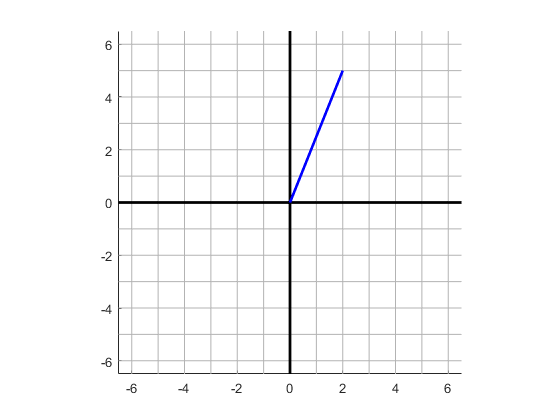
\includegraphics[width=1.4in]{Images/vectorplot25.png}} \quad b)~\parbox[c]{1.4in}{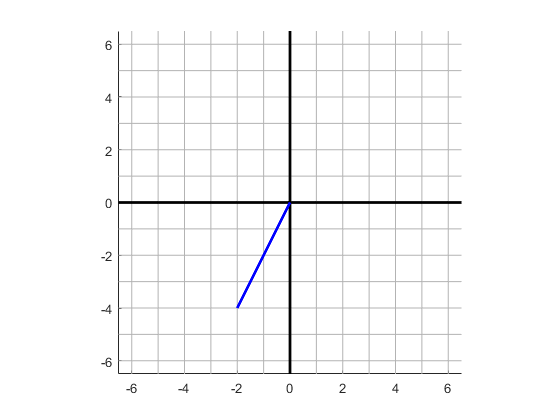
\includegraphics[width=1.4in]{Images/vectorplotm2m4.png}} \quad c)~\parbox[c]{1.4in}{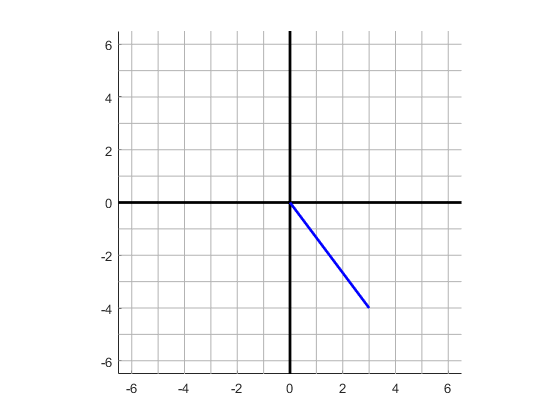
\includegraphics[width=1.4in]{Images/vectorplot3m4.png}}
}

\begin{exercise}
On a piece of graph paper draw the vector $(1,2)$ starting at (based at) the
given point:
\begin{tasks}(3)
\task
based at $(0,0)$
\task
based at $(1,2)$
\task
based at $(0,-1)$
\end{tasks}
\end{exercise}
\comboSol{%
}
{%
a)~\parbox[c]{1.4in}{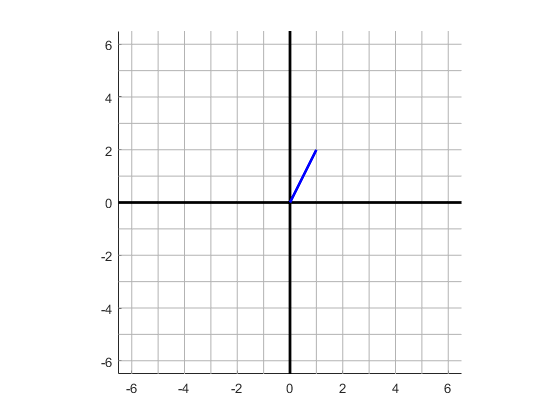
\includegraphics[width=1.4in]{Images/vectorplot1200.png}} \quad b)~\parbox[c]{1.4in}{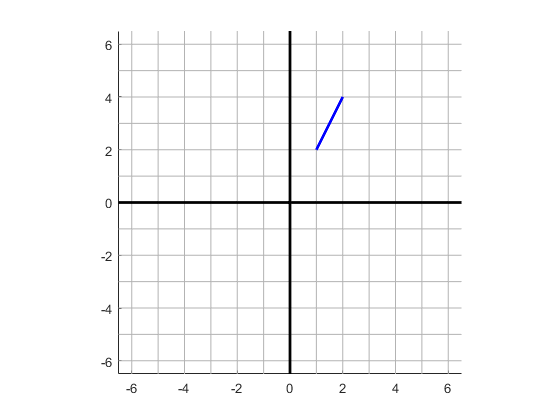
\includegraphics[width=1.4in]{Images/vectorplot1212.png}} \quad c)~\parbox[c]{1.4in}{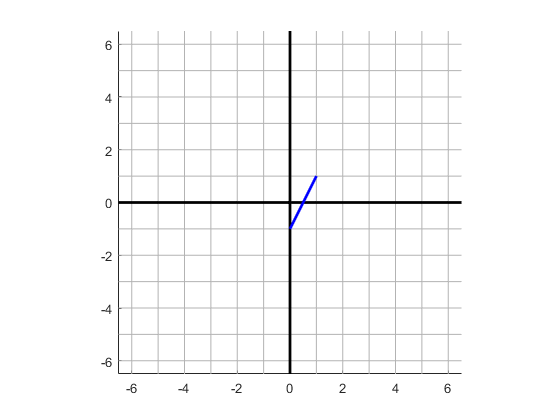
\includegraphics[width=1.4in]{Images/vectorplot120m1.png}}
}

\begin{exercise}
On a piece of graph paper draw the following
operations.  Draw and label the vectors involved in the operations
as well as the result:
\begin{tasks}(3)
\task
$\begin{bmatrix}
1 \\
-4
\end{bmatrix}
+
\begin{bmatrix}
2 \\
3
\end{bmatrix}$
\task
$\begin{bmatrix}
-3 \\
2
\end{bmatrix}
-
\begin{bmatrix}
1 \\
3
\end{bmatrix}$
\task
$3\begin{bmatrix}
2 \\
1
\end{bmatrix}$
\end{tasks}
\end{exercise}
\comboSol{%
}
{%
a)~\parbox[c]{1.4in}{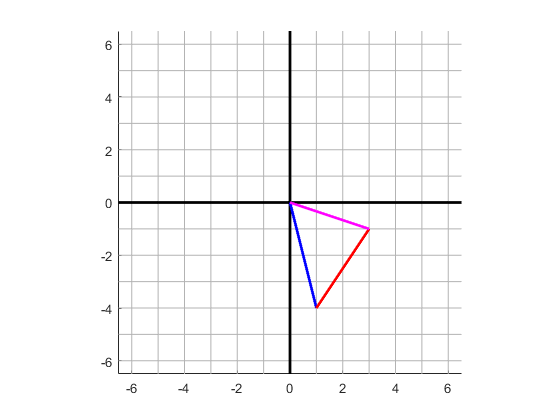
\includegraphics[width=1.4in]{Images/vectorops1.png}} \quad b)~\parbox[c]{1.4in}{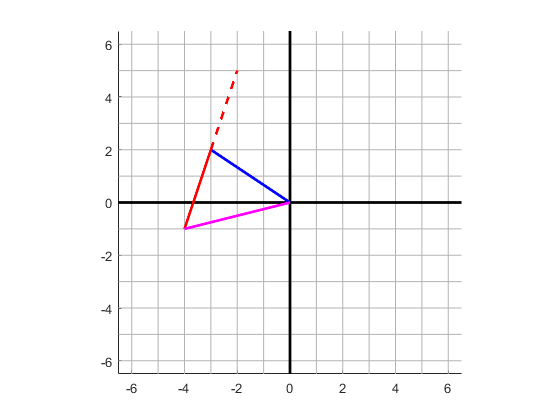
\includegraphics[width=1.4in]{Images/vectorops2.png}} \quad c)~\parbox[c]{1.4in}{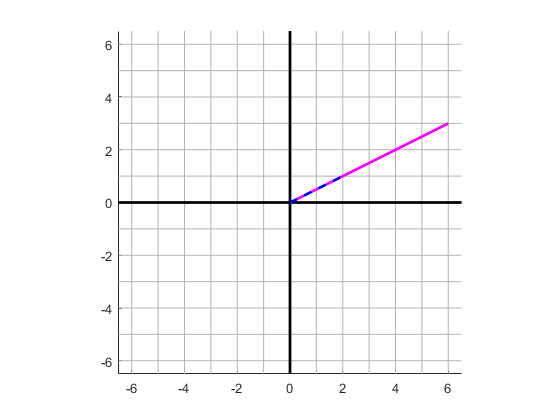
\includegraphics[width=1.4in]{Images/vectorops3.png}}
}

\begin{exercise}
Compute the magnitude of
\begin{tasks}(3)
\task
$\begin{bmatrix}
7 \\
2 
\end{bmatrix}
$
\task
$\begin{bmatrix}
-2 \\
3 \\
1
\end{bmatrix}
$
\task
$(1,3,-4)$
\end{tasks}
\end{exercise}
\comboSol{%
}
{%
a)~ $\sqrt{53}$ \quad b~) $\sqrt{14}$ \quad c)~ $\sqrt{26}$
}

\begin{exercise}\ansMark%
Compute the magnitude of
\begin{tasks}(3)
\task
$\begin{bmatrix}
1 \\
3
\end{bmatrix}
$
\task
$\begin{bmatrix}
2 \\
3 \\
-1
\end{bmatrix}
$
\task
$(-2,1,-2)$
\end{tasks}
\end{exercise}
\exsol{%
a)~$\sqrt{10}$
\quad b)~$\sqrt{14}$
\quad c)~$3$
}

\begin{exercise}
Compute
\begin{tasks}(3)
\task
$\begin{bmatrix}
2 \\
3 
\end{bmatrix}
+
\begin{bmatrix}
7 \\
-8
\end{bmatrix}
$
\task
$\begin{bmatrix}
-2 \\
3 
\end{bmatrix}
-
\begin{bmatrix}
6 \\
-4
\end{bmatrix}
$
\task
$
-\begin{bmatrix}
-3 \\
2 
\end{bmatrix}
$
\task
$
4\begin{bmatrix}
-1 \\
5 
\end{bmatrix}
$
\task
$
5\begin{bmatrix}
1 \\
0 
\end{bmatrix}
+
9
\begin{bmatrix}
0 \\
1
\end{bmatrix}
$
\task
$
3\begin{bmatrix}
1 \\
-8 
\end{bmatrix}
-
2
\begin{bmatrix}
3 \\
-1
\end{bmatrix}
$
\end{tasks}
\end{exercise}
\comboSol{%
}
{%
a) $\left[\begin{smallmatrix} 9 \\ -5 \end{smallmatrix}\right]$ \quad b)~ $\left[\begin{smallmatrix}  -8 \\ 7 \end{smallmatrix}\right]$ \quad c)~ $\left[\begin{smallmatrix} 3 \\ -2 \end{smallmatrix}\right]$ \quad
d)~ $\left[\begin{smallmatrix} -4 \\ 20 \end{smallmatrix}\right]$ \quad e)~ $\left[\begin{smallmatrix} 5 \\ 9 \end{smallmatrix}\right]$ \quad f)~ $\left[\begin{smallmatrix} -3 \\ -22 \end{smallmatrix}\right]$
}

\begin{exercise}\ansMark%
\pagebreak[2]
Compute
\begin{tasks}(3)
\task
$\begin{bmatrix}
3 \\
1 
\end{bmatrix}
+
\begin{bmatrix}
6 \\
-3
\end{bmatrix}
$
\task
$\begin{bmatrix}
-1 \\
2 
\end{bmatrix}
-
\begin{bmatrix}
2 \\
-1
\end{bmatrix}
$
\task
$
-\begin{bmatrix}
-5 \\
3 
\end{bmatrix}
$
\task
$
2\begin{bmatrix}
-2 \\
4 
\end{bmatrix}
$
\task
$
3\begin{bmatrix}
1 \\
0 
\end{bmatrix}
+
7
\begin{bmatrix}
0 \\
1
\end{bmatrix}
$
\task
$
2\begin{bmatrix}
2 \\
-3 
\end{bmatrix}
-
6
\begin{bmatrix}
2 \\
-1
\end{bmatrix}
$
\end{tasks}
\end{exercise}
\exsol{%
a)~$\left[\begin{smallmatrix}
9 \\
-2
\end{smallmatrix}\right]$
\quad b)~$\left[\begin{smallmatrix}
-3 \\
3
\end{smallmatrix}\right]$
\quad c)~$\left[\begin{smallmatrix}
5 \\
-3
\end{smallmatrix}\right]$
\quad d)~$\left[\begin{smallmatrix}
-4 \\
8
\end{smallmatrix}\right]$
\quad e)~$\left[\begin{smallmatrix}
3 \\
7
\end{smallmatrix}\right]$
\quad f)~$\left[\begin{smallmatrix}
-8 \\
0
\end{smallmatrix}\right]$
}

\begin{exercise}
Find the unit vector in the direction of the given vector
\begin{tasks}(3)
\task
$\begin{bmatrix}
1 \\
-3 
\end{bmatrix}
$
\task
$\begin{bmatrix}
2 \\
1 \\
-1
\end{bmatrix}
$
\task
$(3,1,-2)$
\end{tasks}
\end{exercise}
\comboSol{%
}
{%
a)~$\left[\begin{smallmatrix} 1/\sqrt{10} \\ -3/\sqrt{10} \end{smallmatrix}\right]$ \quad b)~ $\left[\begin{smallmatrix} 2/\sqrt{6} \\ 1/\sqrt{6} \\ -1/\sqrt{6} \end{smallmatrix}\right]$ \quad c)~ $\left( \frac{3}{\sqrt{14}}, \frac{1}{\sqrt{14}}, -\frac{2}{\sqrt{14}}\right)$
}

\begin{exercise}\ansMark%
Find the unit vector in the direction of the given vector
\begin{tasks}(3)
\task
$\begin{bmatrix}
-1 \\
1 
\end{bmatrix}
$
\task
$\begin{bmatrix}
1 \\
-1 \\
2
\end{bmatrix}
$
\task
$(2,-5,2)$
\end{tasks}
\end{exercise}
\exsol{%
a)~
$\left[\begin{smallmatrix}
\frac{-1}{\sqrt{2}} \\
\frac{1}{\sqrt{2}}
\end{smallmatrix}\right]$
\quad
b)~$\left[\begin{smallmatrix}
\frac{1}{\sqrt{6}} \\
\frac{-1}{\sqrt{6}} \\
\frac{2}{\sqrt{6}}
\end{smallmatrix}\right]$
\quad
c)~$\left( \frac{2}{\sqrt{33}},\frac{-5}{\sqrt{33}},\frac{2}{\sqrt{33}} \right)$
}

\begin{exercise}
If $\vec{x} = (1,2)$ and $\vec{y}$ are added together, we find
$\vec{x}+\vec{y} = (0,2)$.  What is $\vec{y}$?
\end{exercise}
\comboSol{%
}
{%
$\begin{bmatrix}  -1 \\ 0  \end{bmatrix}$
}

\begin{exercise}
If $\vec{v} = (1, -4, 3)$ and $\vec{w} = (-2, 3, -1)$, compute $3\vec{v} - 2\vec{w}$ and $4\vec{w} + \vec{v}$. 
\end{exercise}
\comboSol{%
}
{%
$(9, -18, 11)$, $(-7, 8, -1)$
}

\begin{exercise}
Write $(1,2,3)$ as a linear combination of the standard basis vectors
$\vec{e}_1$, $\vec{e}_2$, and $\vec{e}_3$.
\end{exercise}
\comboSol{%
}
{%
$1\vec{e}_1 + 2\vec{e}_2 + 3\vec{e}_3$
}

\begin{exercise}
Determine if the following sets of vectors are linearly independent.
\begin{tasks}(2)
\task $\displaystyle \left\{ \begin{bmatrix} 1 \\ 1 \end{bmatrix},\ \begin{bmatrix} 0 \\ 1 \end{bmatrix}\right\}$
\task $\displaystyle \left\{ \begin{bmatrix} 1 \\ 1 \\ 1 \end{bmatrix},\ \begin{bmatrix} 2 \\ 2 \\ 2 \end{bmatrix} \right\}$
\task $\displaystyle \left\{ \begin{bmatrix} 1 \\ 2 \end{bmatrix},\ \begin{bmatrix} -1 \\ 3 \end{bmatrix},\ \begin{bmatrix}  1 \\ 1 \end{bmatrix}\right\}$
\task $\displaystyle \left\{ \begin{bmatrix}  1 \\ 0 \end{bmatrix},\ \begin{bmatrix} 0 \\ 0 \end{bmatrix}\right\}$
\task $\displaystyle \left\{ \begin{bmatrix} 1 \\ 0 \\ 0 \end{bmatrix},\ \begin{bmatrix} 0 \\ 1 \\ -1 \end{bmatrix},\ \begin{bmatrix} 0 \\ 0 \\ 2 \end{bmatrix}\right\}$
\task $\displaystyle \left\{ \begin{bmatrix} 0 \\ 1 \\ 0 \end{bmatrix},\ \begin{bmatrix} 0 \\ 3 \\ -1 \end{bmatrix},\ \begin{bmatrix} 0 \\ -2 \\ 1 \end{bmatrix}\right\}$
\end{tasks}
\end{exercise}
\comboSol{%
}
{%
a)~Yes \quad b)~No \quad c)~No \quad d)~No \quad e)~Yes \quad f)~No
}


\begin{exercise}
If the magnitude of $\vec{x}$ is 4, what is the magnitude of
\begin{tasks}(6)
\task
$0\vec{x}$
\task
$3\vec{x}$
\task
$-\vec{x}$
\task
$-4\vec{x}$
\task
$\vec{x}+\vec{x}$
\task
$\vec{x}-\vec{x}$
\end{tasks}
\end{exercise}
\comboSol{%
}
{%
a)~ 0 \quad b)~ 12 \quad c)~ 4 \quad d)~ 16 \quad e)~ 8 \quad f)~ 0
}

\begin{exercise}\ansMark%
If the magnitude of $\vec{x}$ is 5, what is the magnitude of
\begin{tasks}(3)
\task
$4\vec{x}$
\task
$-2\vec{x}$
\task
$-4\vec{x}$
\end{tasks}
\end{exercise}
\exsol{%
a)~$20$
\quad b)~$10$
\quad c)~$20$
}

\begin{exercise}
Suppose a linear mapping $F \colon {\mathbb R}^2 \to {\mathbb R}^2$
takes $(1,0)$ to $(2,-1)$ and it takes $(0,1)$ to $(3,3)$. 
Where does it take
\begin{tasks}(3)
\task
$(1,1)$
\task
$(2,0)$
\task
$(2,-1)$
\end{tasks}
\end{exercise}
\comboSol{%
}
{%
a)~$(5,2)$ \quad b)~$(4, -2)$ \quad c)~$(7,1)$
}

\begin{exercise}
Suppose a linear mapping $F \colon {\mathbb R}^3 \to {\mathbb R}^2$
takes $(1,0,0)$ to $(2,1)$ and it takes $(0,1,0)$ to $(3,4)$ and
it takes $(0,0,1)$ to $(5,6)$.  Write down the matrix representing
the mapping $F$.
\end{exercise}
\comboSol{%
}
{%
$\left[\begin{smallmatrix} 2 & 3 & 5 \\ 1 & 4 & 6 \end{smallmatrix}\right]$
}

\begin{exercise}
Suppose that a mapping $F \colon {\mathbb R}^2 \to \mathbb{R}^2$ takes
$(1,0)$ to $(1,2)$, $(0,1)$ to $(3,4)$, and it takes $(1,1)$ to $(0,-1)$.
Explain why $F$ is not linear.
\end{exercise}
\comboSol{%
}
{%
$F\left(\left[\begin{smallmatrix} 1 \\ 0 \end{smallmatrix}\right]\right) + F\left(\left[\begin{smallmatrix} 0 \\ 1 \end{smallmatrix}\right]\right) \neq F\left(\left[\begin{smallmatrix} 1 \\ 1 \end{smallmatrix}\right]\right)$
}

\begin{exercise}\ansMark%
Suppose a linear mapping $F \colon {\mathbb R}^2 \to {\mathbb R}^2$
takes $(1,0)$ to $(1,-1)$ and it takes $(0,1)$ to $(2,0)$. 
Where does it take
\begin{tasks}(3)
\task
$(1,1)$
\task
$(0,2)$
\task
$(1,-1)$
\end{tasks}
\end{exercise}
\exsol{%
a)~$(3,-1)$ \quad b)~$(4,0)$ \quad c)~$(-1,-1)$
}

\begin{exercise}[challenging]
Let $P$ represent the space of quadratic polynomials
in $t$: a point $(a_0,a_1,a_2)$ in $P$ represents
the polynomial $a_0 + a_1 t + a_2 t^2$.
Consider the derivative $\frac{d}{dt}$ as a mapping of $P$ to
$P$,
and note that $\frac{d}{dt}$ is linear.
Write down $\frac{d}{dt}$ as a $3 \times 3$ matrix.
\end{exercise}
\comboSol{%
}
{%
$\left[\begin{smallmatrix} 0 & 1 & 0 \\ 0 & 0 & 2 \\ 0 & 0 & 0 \end{smallmatrix}\right]$
}

\setcounter{exercise}{100}
